%!TEX program = xelatex
\documentclass[12pt,a4paper]{article}

% ========== 基础包 ==========
\usepackage{ctex}                 % 中文支持
\usepackage{geometry}
\usepackage{amsmath,amssymb,amsfonts}
\usepackage{bm}                   % 粗体数学符号
\usepackage{cases}                % 分段函数
\usepackage{cancel}               % 删除线（数学）
\usepackage{array}
\usepackage{xcolor}
\usepackage{booktabs}
\usepackage{enumitem}
\usepackage{fancyhdr}
\usepackage{titlesec}
\usepackage{longtable}            % 跨页表格
\usepackage{graphicx}             % 插入图片

% hyperref 最后加载
\usepackage[
    colorlinks=true,
    linkcolor=blue!70!black,
    citecolor=gray,
    urlcolor=blue,
    bookmarks=true,
    bookmarksnumbered=true,
    unicode=true
]{hyperref}

% ========== 页面设置 ==========
\geometry{top=2.5cm, bottom=2.5cm, left=2.5cm, right=2.5cm}

% ========== 颜色定义 ==========
\definecolor{annot补贴}{RGB}{180,50,50}
\definecolor{annot购买}{RGB}{200,100,50}
\definecolor{annot改造}{RGB}{220,150,50}
\definecolor{annot电网}{RGB}{150,120,50}
\definecolor{annot能源}{RGB}{50,130,150}
\definecolor{annot移动}{RGB}{100,150,100}
\definecolor{firststage}{RGB}{70,130,180}
\definecolor{secondstage}{RGB}{220,20,60}

% ========== 标题格式 ==========
\titleformat{\section}{\Large\bfseries\heiti}{\thesection}{1em}{}
\titleformat{\subsection}{\large\bfseries\heiti}{\thesubsection}{1em}{}

% ========== 自定义注释命令 ==========
\newcommand{\手批注}[2]{\textcolor{#1}{\text{\kaishu #2}}}
\newcommand{\一阶段}{\textcolor{firststage}{\text{\kaishu （一阶段）}}}
\newcommand{\二阶段}{\textcolor{secondstage}{\text{\kaishu （二阶段）}}}

\begin{document}

% ========== 标题 ==========
\begin{center}
    \Large\bfseries\heiti 港口设备电动化改造两阶段随机规划模型\\[0.8em]
    \normalsize\kaishu 
\end{center}

\section{问题描述}

集装箱码头是物流系统中的关键节点，其中堆场区域是作业效率的主要瓶颈。堆场内的装卸作业主要由场桥（Yard Crane, YC）完成。传统柴油驱动的场桥（Diesel YC, DYC）虽然作业效率较高，但碳排放量大、运营成本高。为响应国家低碳政策与绿色港口建设目标，港口企业逐步将 DYC 改造为电动场桥（Electric YC, EYC），以降低碳排放和长期运营成本。

然而，EYC 的推广面临多重挑战：首先，改造需要堆场区域进行电网铺设，改造期间该区域无法部署 EYC；其次，EYC 的作业效率仅为 DYC 的 $\beta$ 倍（$0<\beta<1$），存在产能损失；此外，改造成本较高，且各堆场区域的作业需求量受船舶到港时间、装卸计划、天气等因素影响，具有显著的不确定性。这种不确定性将直接影响改造与部署策略的制定。

为此，政府提供投资补贴（比例为 $k$），并实施碳排放交易政策（Carbon Emission Trading, CET），以激励企业加速绿色转型。本文采用\textbf{两阶段随机规划}（Two-stage Stochastic Programming）方法建模：
\begin{itemize}[itemsep=0.2em,leftmargin=2em]
    \item \textbf{第一阶段决策}：在需求实现之前就必须确定的基础设施投资决策，包括购买新的 EYC、将 DYC 改造为 EYC、对堆场区域进行电网改造。这些决策一旦做出便不可更改，\textbf{不随随机场景变化}。
    \item \textbf{第二阶段决策}：在观察到具体的随机需求实现后，企业根据手头的设备资源进行的日常调度操作，包括两类设备的作业量分配、DYC 在不同区域之间的移动。这些决策\textbf{随随机场景变化}。
\end{itemize}

企业的目标是\textbf{最小化规划期内总成本的期望值}，包括确定性的投资成本，以及场景期望的运营成本与碳排放超额成本。约束条件涵盖设备数量守恒、供需平衡、预算限制、碳排放配额及设备产能上限。

{SAA 离散近似}

在真实世界中，未来的港口作业需求 $\tilde{h}_{zt}$ 是一个连续型的随机变量，记其真实的概率分布为 $P$。两阶段随机规划的理论目标函数写为包含连续积分的期望值形式：
\begin{equation}
    \min \; C_{\text{inv}} + \mathbb{E}_{\tilde{h}} \Bigl[ C_{\text{op}}(\tilde{h}) + C_{\text{carbon}}(\tilde{h}) \Bigr]
    \label{eq:continuous-expectation}
\end{equation}

其中 $\mathbb{E}_{\tilde{h}}[\cdot]$ 表示关于随机需求 $\tilde{h}$ 的数学期望。

\textbf{样本均值近似法（Sample Average Approximation, SAA）}的核心思想是：通过从连续分布 $P$ 中独立同分布（i.i.d.）地随机抽取 $|S|$ 个场景样本，用样本均值来近似逼近真实的数学期望。由于每个场景是被独立随机抽取的，因此在模型中每个场景发生的概率均等，即 $\pi_s = \frac{1}{|S|}$。

通过 SAA 方法转化后，原问题被写成一个\textbf{确定性等价的大型线性规划模型}，能够直接求解。SAA 的目标函数形式为：
\begin{equation}
    \min \; C_{\text{total}} = C_{\text{inv}} + \frac{1}{|S|} \sum_{s \in S} \left( C_{\text{op},s} + C_{\text{carbon},s} \right)
    \label{eq:saa-approximation}
\end{equation}

为方便起见，下文中 DYC、EYC 两类设备分别记为设备1、设备2。假设共有 $|S|$ 个等概率场景。

% ============================================================
\section{两阶段决策变量划分}
% ============================================================

\subsection{第一阶段决策变量}

第一阶段决策在需求实现之前做出，\textbf{不随场景变化}：

\begin{itemize}[itemsep=0.2em,leftmargin=2em]
    \item $b_{2zt}$：区域 $z$ 在时段 $t$ 的设备2（EYC）购买量
    \item $y_{zt}$：区域 $z$ 在时段 $t$ 的设备改造量（DYC $\to$ EYC）
    \item $a_{zt} \in \{0,1\}$：区域 $z$ 在时段 $t$ 的电网改造指示
    \item $r_{zt} \in \{0,1\}$：区域 $z$ 在时段 $t$ 的电网改造完成指示
    \item $x_{2zt}$：区域 $z$ 在时段 $t$ 的设备2（EYC）保有量
\end{itemize}

\subsection{第二阶段决策变量}

第二阶段决策在观察到具体需求实现后做出，\textbf{随场景 $s \in S$ 变化}：

\begin{itemize}[itemsep=0.2em,leftmargin=2em]
    \item $w_{1zts}$：区域 $z$ 在时段 $t$、场景 $s$ 下设备1（DYC）的作业量
    \item $w_{2zts}$：区域 $z$ 在时段 $t$、场景 $s$ 下设备2（EYC）的作业量
    \item $m_{zz'ts}$：时段 $t$、场景 $s$ 下设备1从区域 $z$ 移动到 $z'$ 的数量
    \item $x_{1zts}$：区域 $z$ 在时段 $t$、场景 $s$ 下的设备1（DYC）保有量
    \item $E_{ns}$：第 $n$ 个周期、场景 $s$ 下的总碳排放量
    \item $\Delta E_{ns}$：第 $n$ 个周期、场景 $s$ 下的超额碳排放量
\end{itemize}

% ============================================================
\section{目标函数}
% ============================================================

总成本由确定性的投资成本与场景期望的运营成本、碳排放成本构成：
\begin{equation}
    \min \; C_{\text{total}} = C_{\text{inv}} + \frac{1}{|S|} \sum_{s \in S} \left( C_{\text{op},s} + C_{\text{carbon},s} \right)
    \label{eq:obj-stochastic}
\end{equation}

\subsection{投资成本 $C_{\text{inv}}$（一阶段，确定性）}

投资成本为补贴和折现后的设备2购买成本、设备1改造为设备2成本、区域电网改造成本之和，\textbf{不随场景变化}：
\begin{equation}
    C_{\text{inv}} = (1-k) \sum_{t \in T} \rho^{t-1} \sum_{z \in Z} \Bigl(
        \underbrace{p_2 b_{2zt}}_{\text{\手批注{annot购买}{购买}}} +
        \underbrace{v_2 y_{zt}}_{\text{\手批注{annot改造}{改造}}} +
        \underbrace{d \, a_{zt}}_{\text{\手批注{annot电网}{电网}}}
    \Bigr)
    \quad \text{（\手批注{annot补贴}{补贴：比例 $k$）}}
\end{equation}

\textbf{变量说明：}
\begin{itemize}[itemsep=0.2em,leftmargin=2em]
    \item $k$：补贴比例；$\rho$：折现率；$p_2$：购买单价
    \item $b_{2zt}$：区域 $z$ 在时段 $t$ 的设备2购买量
    \item $v_2$：设备改造单位成本；$y_{zt}$：设备改造决策变量
    \item $d$：电网改造成本系数；$a_{zt}$：电网改造决策变量
\end{itemize}

\subsection{运营成本 $C_{\text{op},s}$（二阶段，场景依赖）}

运营成本为折旧后的能源成本、设备1移动成本之和，\textbf{随场景 $s$ 变化}：
\begin{equation}
    C_{\text{op},s} = \sum_{t \in T} \rho^{t-1} \sum_{z \in Z} \Bigl(
        \underbrace{o_1 w_{1zts} + o_2 w_{2zts}}_{\text{\手批注{annot能源}{能源}}} +
        \underbrace{\sum_{z' \in Z} u_{zz'} \, m_{zz'ts}}_{\text{\手批注{annot移动}{移动}}}
    \Bigr)
\end{equation}

\textbf{变量说明：}
\begin{itemize}[itemsep=0.2em,leftmargin=2em]
    \item $o_1, o_2$：两类设备的运营成本系数
    \item $w_{1zts}, w_{2zts}$：区域 $z$ 在时段 $t$、场景 $s$ 下两类设备工作量
    \item $u_{zz'}$：设备1从区域 $z$ 到 $z'$ 的单位移动成本
    \item $m_{zz'ts}$：时段 $t$、场景 $s$ 下设备1从区域 $z$ 移动到 $z'$ 的量
\end{itemize}

\subsection{碳排放成本 $C_{\text{carbon},s}$（二阶段，场景依赖）}

碳排放成本为折现后的超额碳排放成本（按年计算），\textbf{随场景 $s$ 变化}：
\begin{equation}
    C_{\text{carbon},s} = \sum_{n \in N} \rho^{12n-1} \, c_{\text{etp}} \cdot \Delta E_{ns}
    \label{eq:carbon-s}
\end{equation}

\textbf{变量说明：}
\begin{itemize}[itemsep=0.2em,leftmargin=2em]
    \item $c_{\text{etp}}$：超额碳排放单位成本（元/吨）
    \item $\Delta E_{ns}$：第 $n$ 周期、场景 $s$ 下的超额碳排放量（吨）
    \item $n \in N$：第 $n$ 个周期（每年12个月）
    \item $\pi_s$：场景 $s$ 的发生概率（SAA 下 $\pi_s = 1/|S|$）
\end{itemize}

% ============================================================
\newpage
\section{约束条件}
% ============================================================

本节将约束条件按决策阶段分组：\textbf{第一阶段约束}仅涉及一阶段决策变量，不随场景变化；\textbf{第二阶段约束}涉及二阶段决策变量，每个场景 $s \in S$ 均需独立满足。

\subsection{第一阶段约束}

以下约束仅涉及第一阶段决策变量，\textbf{在所有场景下共享同一组决策}。

\subsubsection{预算约束}

每期购买、设备改造、区域电网改造的花费不超过对应预算上限：
\begin{align}
    \sum_{z \in Z} p_2 \, b_{2zt} &\leq \theta_t, && \forall \, t \in T
    \label{eq:budget1-s} \\[6pt]
    \sum_{z \in Z} v_2 \, y_{zt} &\leq \mu_t, && \forall \, t \in T
    \label{eq:budget2-s} \\[6pt]
    \sum_{z \in Z} d \cdot a_{zt} &\leq q_t, && \forall \, t \in T
    \label{eq:budget3-s}
\end{align}
其中 $\theta_t$、$\mu_t$、$q_t$ 分别为购买、设备改造、区域电网改造的预算上限。

\subsubsection{类型 2 设备动态守恒}

类型2设备（EYC）存量仅由购买和改造决定，不随场景变化：
\begin{equation}
    x_{2zt} = 
    \begin{cases}
        x_{2,z,t-1} + b_{2zt} + y_{z,t-\tau}, & \forall \, z \in Z, \; t > \tau \\[6pt]
        x_{2,z,t-1} + b_{2zt}, & \forall \, z \in Z, \; t \leq \tau
    \end{cases}
    \label{eq:dyn2-s}
\end{equation}

初始条件：
\begin{equation}
    x_{2,z,0} = 0, \qquad \forall \, z \in Z
    \label{eq:dyn2_init-s}
\end{equation}

$t$ 期 $z$ 区域的设备2数量取决于上期设备2数量、本期设备2购买量、以及 $\tau$ 期前启动的改造在本期完成的数量。

\subsubsection{电网改造约束}

每个区域最多改造一次电网：
\begin{equation}
    \sum_{t \in T} a_{zt} \leq 1, \qquad \forall \, z \in Z
    \label{eq:reform_once-s}
\end{equation}

电网改造完成标记：
\begin{equation}
    r_{zt} = \sum_{t'=1}^{t-t_z} a_{zt'},
    \qquad \forall \, z \in Z, \; t > t_z
    \label{eq:reform_cumul-s}
\end{equation}
\begin{equation}   
    r_{zt} = 0, \qquad \forall z \in Z, \; t \leq t_z
    \label{eq:reform_zero-s}
\end{equation}

\subsubsection{类型 2 设备容量上限}

电网改造完成后才允许部署设备2：
\begin{equation}
    x_{2zt} \leq m_z \cdot r_{zt}, \qquad \forall \, z \in Z, \; t \in T
    \label{eq:cap_type2-s}
\end{equation}

% ============================================================
\subsection{第二阶段约束（Wait-and-See）}

以下约束涉及第二阶段决策变量，\textbf{对每个场景 $s \in S$ 均需独立满足}。

\subsubsection{供需平衡约束}

各场景下，区域 $z$ 在时段 $t$ 的两类设备作业量之和等于该场景的需求量：
\begin{equation}
    w_{1zts} + w_{2zts} = h_{zts}, \qquad \forall \, z \in Z, \; t \in T, \; s \in S
    \label{eq:balance-s}
\end{equation}

\subsubsection{产能上限约束}

各场景下，作业量不超过对应设备的产能上限（设备1存量 $x_{1zts}$ 随场景变化，设备2存量 $x_{2zt}$ 为一阶段决策）：
\begin{align}
    w_{1zts} &\leq g_1 \, x_{1zts}, && \forall \, z \in Z, \; t \in T, \; s \in S
    \label{eq:cap1-s} \\[6pt]
    w_{2zts} &\leq g_2 \, x_{2zt} = \beta g_1 \, x_{2zt}, && \forall \, z \in Z, \; t \in T, \; s \in S
    \label{eq:cap2-s}
\end{align}

\subsubsection{类型 1 设备动态守恒}

由于设备移动量 $m_{zz'ts}$ 随场景变化，类型1设备存量 $x_{1zts}$ 也必须带上场景索引 $s$：
\begin{equation}
    x_{1zts} = x_{1,z,t-1,s} - y_{zt} + \sum_{z' \in Z} m_{z'zts} - \sum_{z' \in Z} m_{zz'ts},
    \qquad \forall \, z \in Z, \; t > 1, \; s \in S
    \label{eq:dyn1_t-s}
\end{equation}

初始期（$t=1$，各场景共享相同的初始存量 $f_z$）：
\begin{equation}
    x_{1z1s} = f_z - y_{z1} + \sum_{z' \in Z} m_{z'z1s} - \sum_{z' \in Z} m_{zz'1s},
    \qquad \forall \, z \in Z, \; s \in S
    \label{eq:dyn1_init-s}
\end{equation}

改造量不超过当前类型1存量：
\begin{align}
    y_{zt} &\leq x_{1,z,t-1,s}, && \forall \, z \in Z, \; t > 1, \; s \in S
    \label{eq:y-le-x1-s} \\[6pt]
    y_{z1} &\leq f_z, && \forall \, z \in Z
    \label{eq:y-le-f-s}
\end{align}

\subsubsection{碳排放约束}

各场景下各周期总排放量：
\begin{equation}
    E_{ns} = \sum_{t=12(n-1)+1}^{12n} \sum_{z \in Z}
    \frac{1}{1000} \left( e_1 \, w_{1zts} + e_2 \, w_{2zts} \right),
    \qquad \forall \, n \in N, \; s \in S
    \label{eq:emission-s}
\end{equation}

各场景下排放量削减约束：
\begin{align}
    \Delta E_{ns} &\geq E_{ns} - c_{\text{feqp}} \, E_{n-1,s}, && \forall \, n > 1, \; s \in S
    \label{eq:cut1-s} \\[6pt]
    \Delta E_{1s} &\geq E_{1s} - Q_1, && \forall \, s \in S
    \label{eq:cut2-s} \\[6pt]
    \Delta E_{ns} &\geq 0, && \forall \, n \in N, \; s \in S
    \label{eq:cut3-s}
\end{align}

$c_{\text{feqp}}$ 为排放削减系数，$Q_1$ 为第一年排放基准。

\subsubsection{总设备数量上限}

各场景下，两类设备存量之和不超过区域容量上限：
\begin{equation}
    x_{1zts} + x_{2zt} \leq m_z, \qquad \forall \, z \in Z, \; t \in T, \; s \in S
    \label{eq:cap_total-s}
\end{equation}

其中 $m_z$ 为区域 $z$ 的设备容量上限。

\vspace{0.8em}
\noindent\textbf{需求分布设定。}各区域各时段的作业需求 $\tilde{h}_{zt}$ 为连续型随机变量。由于港口作业量天然非负且存在"抢出口"、节前备货等极端高需求场景（右偏分布），本模型采用\textbf{对数正态分布}刻画需求不确定性。具体地，各时段需求按下式生成场景样本：
\begin{equation}
    h_{zts} \sim \text{LogNormal}\left(\ln(\mu_{zt}) - \frac{\sigma^2}{2},\; \sigma^2\right), \qquad \sigma = \sqrt{\ln(1 + \text{CV}^2)}
    \label{eq:lognormal-param}
\end{equation}

其中基准均值 $\mu_{zt}$ 融合历史月均吞吐量与季节性因子：
\begin{equation}
    \mu_{zt} = \bar{h}_z \times \text{season}_t
    \label{eq:seasonal}
\end{equation}

季节性因子 season$_t$ 建议取值如下：
\begin{itemize}[itemsep=0.1em,leftmargin=2em]
    \item 2月（春节）：0.75 $\sim$ 0.85
    \item 5~7月（淡季）：0.90 $\sim$ 0.95
    \item 8~10月（旺季）：1.05 $\sim$ 1.10
    \item 11~12月（圣诞备货高峰）：1.15 $\sim$ 1.25
    \item 其他月份：0.95 $\sim$ 1.00
\end{itemize}

$\bar{h}_z$ 为区域 $z$ 的历史年均吞吐量除以12。

% ============================================================
\newpage
\section{符号汇总表}
% ============================================================

\begin{footnotesize}
\renewcommand{\arraystretch}{1.15}
\begin{longtable}{clp{7.5cm}}
\toprule
\textbf{符号} & \textbf{含义} & \textbf{备注} \\
\midrule
\endfirsthead
\toprule
\textbf{符号} & \textbf{含义} & \textbf{备注} \\
\midrule
\endhead
\bottomrule
\endfoot
\multicolumn{3}{l}{\textbf{集合}} \\
$Z$ & 区域集合 & $z \in Z$ 为区域索引 \\
$T$ & 时段集合 & $t \in T$ 为时段索引 \\
$N$ & 周期集合 & $n \in N$ 为年度周期（每周期12期） \\
$S$ & 场景集合 & $s \in S$ 为随机场景索引（SAA采样） \\
\midrule
\multicolumn{3}{l}{\textbf{参数}} \\
$k$ & 补贴比例 & 投资成本补贴率 \\
$\rho$ & 折现率 & $\rho^{t-1}$ 为第 $t$ 期折现因子 \\
$p_2$ & 购买单价 & 类型2设备单位购买价格 \\
$v_2$ & 改造成本 & 设备改造单位成本 \\
$d$ & 电网成本系数 & 电网接入相关成本系数 \\
$o_1, o_2$ & 运营成本系数 & 两类设备的单位运营成本 \\
$u_{zz'}$ & 移动成本 & 从区域 $z$ 到 $z'$ 的单位运输/移动成本 \\
$g_1, g_2$ & 产能系数 & 两类设备的单位产能（$g_2 = \beta g_1$） \\
$e_1, e_2$ & 排放系数 & 两类设备的单位碳排放系数 \\
$c_{\text{feqp}}$ & 排放削减系数 & 碳排放年削减系数 \\
$c_{\text{etp}}$ & 超额排放成本系数 & 碳排放超额部分单价系数 \\
$\tau$ & 改造时滞 & 改造生效前的延迟期数 \\
$t_z$ & 改造完成时间 & 区域 $z$ 的改造完成时点 \\
$m_z$ & 容量上限 & 区域 $z$ 的设备总容量上限 \\
$f_z$ & 初始存量 & 区域 $z$ 的类型1设备初始数量 \\
$\theta_t$ & 购买预算约束 & 时间 $t$ 购买设备2的预算约束 \\
$\mu_t$ & 改造预算约束 & 时间 $t$ 设备改造成设备2的预算约束 \\
$q_t$ & 电网改造预算约束 & 时间 $t$ 的区域电网改造预算约束 \\
$Q_1$ & 初始碳排放免费额度 & $t=1$ 期的碳排放免费额度 \\
$h_{zts}$ & 作业总需求 & 区域 $z$ 在时间 $t$、场景 $s$ 的作业需求 \\
$\pi_s$ & 场景概率 & 场景 $s$ 的发生概率（SAA下$\pi_s=1/|S|$） \\
\midrule
\multicolumn{3}{l}{\textbf{一阶段决策变量（不随场景变化）}} \\
$b_{2zt}$ & 购买量 & 区域 $z$ 在时段 $t$ 的类型2设备购买量 \\
$y_{zt}$ & 改造量 & 区域 $z$ 在时段 $t$ 的改造设备数量 \\
$a_{zt}$ & 电网改造指示 & $a_{zt} \in \{0,1\}$，是否进行电网改造 \\
$r_{zt}$ & 电网改造完成指示 & $r_{zt} \in \{0,1\}$，是否完成电网改造 \\
$x_{2zt}$ & 设备2存量 & 区域 $z$ 在时段 $t$ 的类型2设备保有量 \\
\midrule
\multicolumn{3}{l}{\textbf{二阶段决策变量（随场景变化）}} \\
$w_{1zts}$ & 设备1作业量 & 场景 $s$ 下区域 $z$ 时段 $t$ 的设备1作业量 \\
$w_{2zts}$ & 设备2作业量 & 场景 $s$ 下区域 $z$ 时段 $t$ 的设备2作业量 \\
$m_{zz'ts}$ & 移动量 & 场景 $s$ 下时段 $t$ 设备1从 $z$ 移到 $z'$ 的数量 \\
$x_{1zts}$ & 设备1存量 & 场景 $s$ 下区域 $z$ 时段 $t$ 的类型1设备保有量 \\
$E_{ns}$ & 周期排放量 & 场景 $s$ 下第 $n$ 周期的总碳排放量 \\
$\Delta E_{ns}$ & 超额排放量 & 场景 $s$ 下第 $n$ 周期的碳排放超额量 \\
\bottomrule
\end{longtable}
\end{footnotesize}


% ============================================================
\newpage
\section{参数取值说明与数据来源}
% ============================================================

本节详细说明模型中所有参数的取值依据。

\begin{footnotesize}
\renewcommand{\arraystretch}{1.2}
\begin{longtable}{clp{10cm}}
\toprule
\textbf{参数} & \textbf{取值} & \textbf{来源/依据}\\
\midrule
\endfirsthead
\toprule
\textbf{参数} & \textbf{取值} & \textbf{来源/依据}\\
\midrule
\endhead
\bottomrule
\endfoot

\multicolumn{3}{l}{\textbf{一、碳排放与交易政策参数}} \\
\midrule
$c_{\text{etp}}$ & 65 元/吨 & 生态环境部：2025年全国碳市场全年交易均价62.36元/吨$^{[1]}$\\
$c_{\text{feqp}}$ & 0.70 & 生态环境部：2023、2024 年度各机组预分配配额量均为该机组上一年度经核查排放量的 70\%$^{[2]}$ \\
$Q_1$ & 645 吨 & 第一年初始免费额度，结合生态环境部规定推算$^{[2]}$ \\
$e_1$（DYC） & 3.2 kg CO$_2$/TEU & GLEC 3.1框架：柴油TTW排放73.8 g CO$_2$e/MJ；实测DYC柴油消耗约1.2 L/TEU，换算得3.2 kg CO$_2$/TEU$^{[3]}$  \\
$e_2$（EYC） & 1.4 kg CO$_2$/TEU & 中国电网电力WTW排放158.4 g CO$_2$e/MJ；实测EYC电力消耗约2.5 kWh/TEU，按电网因子0.5703 kg/kWh换算$^{[3]}$ \\

\midrule
\multicolumn{3}{l}{\textbf{二、投资与改造成本参数}} \\
\midrule
$v_2$ & 50 万元/台 & 天高高科：RTG低空滑触线改造成本45-60万/台，高空滑触线80-96万/台$^{[4]}$，取更通用的低空滑触线改造成本50万/台 \\
$p_2$ & 75 万元/台 & 新购ERTG比改造贵，但无精确公开报价。参考改造成本（50万）和一般工程经验，假设购买单价约为改造的1.5倍\\
$d$ & 50 万元/区域 & 堆场区域电网铺设（含设计、施工、调试）无精确公开报价，假设50万/区域 \\
$k$ & 0.2 & 长江经济带岸电改造中央预算内资金"不超过项目总投资60\%"$^{[5]}$。实际执行比例无公开数据，假设实际补贴比例约20\% \\

\midrule
\multicolumn{3}{l}{\textbf{三、运营效率参数}} \\
\midrule
$o_1$（DYC） & 5.0 元/TEU & 上海特钢设备协会实测：轮胎吊采用柴油发电机成本4.74元/TEU$^{[6]}$，取整为5.0\\
$o_2$（EYC） & 3.0 元/TEU & 上海特钢设备协会实测：轮胎吊采用滑触线供电成本1.00元/TEU$^{[6]}$。但考虑设备维护、电网损耗等综合因素，取3.0（为DYC的60\%） \\
$g_1$ & 3,250 TEU/台$\cdot$月 & RTG作业效率每小时20-30自然箱，月工作约200小时，考虑利用率60\%~70\%，折合 3,250 TEU/台$\cdot$月$^{[7]}$ \\
$\beta$ & 0.80 & 课程设定：EYC作业效率为DYC的$\beta$倍（$0<\beta<1$） \\
$g_2$ & $\beta g_1 = 2,600$ & 由$\beta$和$g_1$推算 \\
$\tau$ & 2 个月 & 单台RTG油改电施工周期约2-4周，考虑批量改造、调试、验收，取2个月 \\
$t_z$ & $\{6,5,4\}$ & 堆场区域电网铺设（滑触线/电缆卷盘）含设计、施工、调试，一般需4-6个月。\\

\midrule
\multicolumn{3}{l}{\textbf{四、容量与预算参数}} \\
\midrule
$m_z$ & $\{15,14,13\}$ & 基于公开堆场数据假设\\
$f_z$ & $\{10,9,8\}$ & 各区域初始DYC存量，与容量上限匹配 \\
$\theta_t$ & 75万 & 时变购买预算 \\
$\mu_t$ & 100万 & 时变改造预算 \\
$q_t$ & 50万 & 电网改造预算\\

\midrule
\multicolumn{3}{l}{\textbf{五、需求参数}} \\
\midrule
$|S|$ & 20 & SAA采样场景数，在计算复杂度和精度间寻求平衡 \\
$\bar{h}_z$ & ${10000,8000,6000}$ & 根据上海港2024年真实集装箱吞吐量数据计算$^{[10]}$\\
$\text{CV}$ & 0.15 & \textbf{经验假设}：港口吞吐量月度波动约$\pm20\%$$^{[8]}$。取CV=0.15（中等不确定性）\\
$\rho$ & 0.99 & 厦门港务集装箱码头项目评估报告：折现率6.91\%-9.28\%$^{[9]}$。取年化折现率约8\%，月度约$\rho \approx 0.993$，取0.99。 \\

\bottomrule
\end{longtable}
\end{footnotesize}

\vspace{0.8em}
\noindent\textbf{需求参数设定。}本节以上海港2024年真实集装箱吞吐量数据为基准，按"全港$\to$子港区$\to$堆场区域"的层级结构拆解，得到各区域各时段的确定性需求均值，再通过对数正态分布引入不确定性。

上海港2024年全年集装箱吞吐量为\textbf{5,151万TEU}，同比增长$+4.8\%$，月均约429万TEU$^{[10]}$。洋山四期自动化码头年吞吐量为 636万TEU，月均约53万TEU。此子港区设61个堆场区域，平均每个堆场月均作业约 8,689 TEU。

模型参数：鉴于本文设定为区域数$|Z|=3$的小码头，月均需求分别设定为$\bar{h}_z={10000,8000,6000}$。

\textbf{引入季节性因子。}基于港口行业经验特征$^{[8]}$，各月季节性因子如下（已归一化使年均值为1.0）：
\begin{center}
\begin{tabular}{c|cccccccccccc}
\toprule
月份 & 1 & 2 & 3 & 4 & 5 & 6 & 7 & 8 & 9 & 10 & 11 & 12 \\
\midrule
因子 & 0.98 & 0.78 & 0.95 & 0.96 & 0.97 & 0.98 & 0.97 & 1.06 & 1.05 & 1.04 & 1.12 & 1.16 \\
\bottomrule
\end{tabular}
\end{center}

\textbf{引入同比增长。}上海港2024年实际同比增速为$+4.8\%$。模型设第1周期（$t=1\sim12$）为基准年，第2周期（$t=13\sim24$）整体需求$\times(1+4.8\%)$。

\textbf{对数正态分布场景采样。}由于港口作业量天然非负且存在"抢出口"等极端高需求场景（右偏分布），采用\textbf{对数正态分布}刻画需求不确定性：
\begin{equation}
    h_{zts} \sim \text{LogNormal}\left(\ln(\mu_{zt}) - \frac{\sigma^2}{2},\; \sigma^2\right), \qquad \sigma = \sqrt{\ln(1 + \text{CV}^2)}
    \label{eq:lognormal}
\end{equation}

其中基准均值 $\mu_{zt} = \bar{h}_z \times \text{season}_t \times (1 + 0.048)^{\mathbf{1}_{t>12}}$，CV$=0.15$（中等不确定性）。

\vspace{1em}
\noindent\textbf{数据来源索引：}
\begin{footnotesize}
\begin{enumerate}[itemsep=0.15em,leftmargin=1.5em,label={[\arabic*]}]
    \item 生态环境部：《全国碳市场发展报告（2025）》，均价62.36元/吨。\\ \url{https://www.mee.gov.cn/ywgz/ydqhbh/wsqtkz/202601/t20260101_1139528.shtml}
    \item 生态环境部：《2023、2024年度配额总量和分配方案》，预分配70\%。\\ \url{https://www.mee.gov.cn/xxgk2018/xxgk/xxgk03/202410/}
    \item GLEC Framework 3.1 中文版（Smart Freight Centre）。
    \item 天高高科：RTG"油改电"技术应用及改造价格，2025年。\\ \url{http://www.tiangaodq.com/pddetaildate/news/detail/20250103_11855425.html}
    \item 湖北省交通运输厅：长江干线港口岸电改造奖励资金管理办法。\\ \url{https://jtt.hubei.gov.cn/ghj/zmhd/zxft/202409/t20240910_5331771.shtml}
    \item 上海特钢设备协会：集装箱轮胎吊滑触线供电节能效果分析。\\ \url{http://www.shtgdqhcx.net/shtgdqhcx_Article_11838978.html}
    \item 新天地港机：集装箱轮胎吊(RTG)技术参数。\\ \url{http://xyqzj.com/product/79-cn.html}
    \item 学术文献：沿海港口集装箱吞吐量季节性波动研究。
    \item 中国资产评估协会：港口行业2024年WACC平均值9.44\%。
    \item 中诚信国际：《中国港口行业展望，2026年2月》，上海港2024年吞吐量5151万TEU。\\ \url{https://pdf.dfcfw.com/pdf/H3_AP202602041819761561_1.pdf}
\end{enumerate}
\end{footnotesize}


% ============================================================
\newpage
\section{两阶段随机规划模型的经济学解释}
% ============================================================

\subsection{阶段划分的经济学解释}

本模型将港口设备电动化决策划分为两个阶段，其核心逻辑在于\textbf{决策的可逆性与信息获取的时序}：

\begin{itemize}[itemsep=0.2em,leftmargin=2em]
    \item \textbf{基础设施投资不可逆}：购买 EYC、改造 DYC、铺设电网等决策涉及大额资本支出，一旦实施难以撤回，属于\textbf{承诺性决策}（commitment decisions）。
    \item \textbf{日常运营调度可调整}：在观察到具体的船舶到港计划、天气状况等需求实现后，企业可以根据手头的设备资源灵活调整作业分配和设备移动，属于\textbf{适应性决策}（adaptive decisions）。
\end{itemize}

\subsection{随机规划 vs 确定性模型的本质差异}

与作业1的确定性模型相比，两阶段随机规划模型的核心优势在于：

\begin{enumerate}[itemsep=0.2em,leftmargin=2em]
    \item \textbf{目标函数变为期望值}：确定性模型仅优化单一需求路径下的成本，而随机规划优化所有可能需求场景下成本的加权平均值，使决策对需求波动具有鲁棒性。
    \item \textbf{一阶段决策承担风险}：购买量和改造量不随场景变化，意味着企业需要为这些决策承担需求不确定性带来的风险——如果实际需求低于预期，购买的设备可能闲置；如果高于预期，则可能面临产能不足。
    \item \textbf{二阶段决策吸收波动}：作业分配和设备移动随场景调整，使得企业可以在给定的一阶段投资决策下，尽可能高效地应对各种需求实现。
\end{enumerate}

\subsection{VSS 与 EEV 的管理洞察}

在数值实验中，可通过以下两个指标量化不确定性的价值：

\begin{itemize}[itemsep=0.2em,leftmargin=2em]
    \item \textbf{EEV（期望值问题的期望结果）}：用需求的场景平均值 $\bar{h}_{zt} = \sum_s \pi_s h_{zts}$ 替代随机需求，求解确定性模型得到一阶段决策，再将其代入各场景计算真实期望成本。EEV 忽略了需求波动，可能导致设备投资不足，在极端高需求场景下面临产能爆仓和巨额碳惩罚。
    \item \textbf{VSS（随机解的价值）}：$\text{VSS} = \text{EEV 的真实期望成本} - \text{随机规划的最优期望成本}$。VSS 度量了"考虑不确定性"所带来的成本节约。若 VSS 显著为正，说明两阶段随机规划相比确定性近似具有明显的经济价值。
\end{itemize}

随机规划模型通常会选择在第一阶段\textbf{适度增加设备投资和电网改造投入}（即"多买一点、早改一点"），虽然增加了确定性投资成本，但能有效降低极端场景下的运营成本和碳排放惩罚，从而实现期望总成本的最小化。

\newpage

% ============================================================

\section{算法设计与数值实验}

% ============================================================

本节对应课程要求中的“根据模型结构设计求解算法，并通过数值实验说明算法求解时间与解的质量”。由于两阶段随机规划模型包含大量场景相关变量，若直接将全部场景一次性放入 Gurobi，模型规模会随场景数线性膨胀，变量数和约束数迅速增加。因此，本文围绕“精确求解、分解求解、启发式快速求解和数据驱动策略搜索”的思路设计多类算法，并将其与 Gurobi 确定性等价模型直接求解结果进行对比。

\subsection{算法设计总体框架}

本文实现并比较以下算法：
\begin{itemize}[itemsep=0.2em,leftmargin=2em]
    \item \textbf{Gurobi 直接求解}：将两阶段随机规划转化为确定性等价模型（Deterministic Equivalent Problem, DEP），作为解质量和求解时间的基准。
    \item \textbf{Benders 分解}：将第一阶段投资决策与第二阶段场景运营决策分离，通过割平面迭代逼近二阶段期望成本。
    \item \textbf{均值指导启发式}：先求解平均需求场景下的确定性模型，固定关键整数决策后再回到全场景模型中评估。
    \item \textbf{列生成/场景生成式算法}：从高压力代表性场景开始求解，逐步加入更多场景，降低一次性建模规模。
    \item \textbf{场景分解算法}：分别求解单场景问题，生成候选第一阶段方案，再将候选方案放回全场景模型中评估。
    \item \textbf{强化学习/数据驱动策略搜索}：基于策略扰动、奖励反馈和探索机制，搜索低成本投资方案。
\end{itemize}

上述算法形成了从精确求解到快速启发式求解的算法体系。其中，Gurobi 直接求解用于提供基准；Benders 分解用于解释和利用两阶段结构；其余启发式算法用于在更短时间内获得高质量可行解。

\subsection{Gurobi 直接求解基准}

Gurobi 直接求解方法将所有场景下的二阶段变量同时放入同一个确定性等价模型中。该方法的优点是建模直接、求解结果可作为高质量基准；缺点是当场景数增加时，变量数量和约束数量会迅速膨胀。

直接求解在本文中的作用包括：
\begin{itemize}[itemsep=0.2em,leftmargin=2em]
    \item 验证两阶段随机规划模型的可行性与正确性；
    \item 为 Benders 分解和各类启发式算法提供目标值对比基准；
    \item 用于计算各算法相对于基准解的相对误差。
\end{itemize}

然而，直接求解无法充分利用“给定第一阶段决策后，各场景二阶段问题相互独立”的结构。当场景规模扩展至数百或数千时，完整确定性等价模型会带来显著的内存压力和求解时间压力。

\subsection{Benders 分解算法}

Benders 分解利用两阶段随机规划的结构，将原问题拆分为主问题和场景子问题。

\textbf{主问题}只包含第一阶段决策变量，包括设备购买量 $b_{2zt}$、设备改造量 $y_{zt}$、电网改造决策 $a_{zt}$、电网完成状态 $r_{zt}$ 以及 EYC 存量 $x_{2zt}$。主问题中引入辅助变量 $\theta_s$ 表示场景 $s$ 的二阶段成本估计。

\textbf{子问题}在给定第一阶段决策后，对每个场景 $s$ 独立求解运营调度问题，包括作业量分配、DYC 移动、设备存量平衡和碳排放成本结算。如果子问题最优，则根据对偶变量生成最优性割；如果子问题不可行，则根据极射线生成可行性割。

\subsubsection{Benders 分解伪代码}

\begin{enumerate}[itemsep=0.2em,leftmargin=2em]
    \item 初始化主问题，仅包含第一阶段变量、第一阶段约束以及二阶段成本估计变量 $\theta_s$。
    \item 求解主问题，得到第一阶段解 $\bar{x}$，包括 $\bar{b}_{2zt}$、$\bar{y}_{zt}$、$\bar{a}_{zt}$ 和 $\bar{x}_{2zt}$。
    \item 对每个场景 $s \in S$：
    \begin{enumerate}[itemsep=0.1em,leftmargin=2em]
        \item 固定第一阶段解 $\bar{x}$；
        \item 求解场景子问题 $SP_s$；
        \item 若 $SP_s$ 可行且最优，则利用对偶变量生成最优性割；
        \item 若 $SP_s$ 不可行，则利用 Farkas 极射线生成可行性割。
    \end{enumerate}
    \item 将新生成的割加入主问题。
    \item 更新下界 $LB$ 和上界 $UB$。
    \item 若 $(UB-LB)/LB \leq \varepsilon$，则算法收敛；否则返回第2步。
    \item 输出最优或近似最优的第一阶段投资方案与期望总成本。
\end{enumerate}

\subsubsection{Benders 分解绕过直接求解瓶颈的机制}

Gurobi 直接求解的主要瓶颈在于所有场景变量和约束必须同时进入一个完整模型。Benders 分解通过以下方式缓解这一问题：
\begin{itemize}[itemsep=0.2em,leftmargin=2em]
    \item \textbf{空间解耦}：每个场景子问题独立求解，单个子问题规模远小于完整 DEP 模型。
    \item \textbf{迭代逼近}：主问题不显式包含完整二阶段约束，而是通过割平面逐步逼近二阶段价值函数。
    \item \textbf{多割策略}：每个场景分别生成 $\theta_s$ 的割，一轮迭代可同时加入多个场景割。
    \item \textbf{并行潜力}：不同场景子问题相互独立，未来可并行求解，从而适应更大规模场景集。
\end{itemize}

因此，Benders 分解并非简单替代 Gurobi，而是利用问题结构将一个整体大模型拆成多个小模型，通过“主问题--子问题--割平面”的迭代过程降低内存压力并提升可扩展性。

\subsection{均值指导启发式算法}

均值指导启发式算法的核心思想是：先将所有需求场景取平均，构造平均需求场景下的确定性模型；再将该模型得到的关键第一阶段整数变量用于指导全场景模型。

算法步骤如下：
\begin{enumerate}[itemsep=0.2em,leftmargin=2em]
    \item 计算各区域各时段的平均需求 $\bar{h}_{zt}=\frac{1}{|S|}\sum_{s\in S}h_{zts}$。
    \item 基于平均需求构建确定性模型并求解。
    \item 提取电网改造决策 $a_{zt}$、设备购买决策 $b_{2zt}$ 和设备改造决策 $y_{zt}$。
    \item 将关键整数变量 $a_{zt}$ 固定为平均需求模型的解。
    \item 回到全场景模型中优化剩余变量，并评估真实期望总成本。
\end{enumerate}

该算法的优点是速度极快，适合在实际运营中快速生成高质量可行解；局限是平均场景可能低估极端高需求风险，因此需要与随机规划精确解进行对比。

\subsection{列生成/场景生成式算法}

列生成思想在本文中体现为“场景生成式算法”：不一次性纳入所有场景，而是从代表性高压力场景开始求解，再逐步加入更多场景。

算法步骤如下：
\begin{enumerate}[itemsep=0.2em,leftmargin=2em]
    \item 对每个场景计算压力分数，综合考虑总需求量和相对峰值需求。
    \item 选择少量高压力场景构建缩减随机规划模型。
    \item 求解缩减模型，得到第一阶段投资方案。
    \item 固定该第一阶段方案，在全场景模型中评估真实期望成本。
    \item 继续加入更多高压力场景，重复求解和评估。
    \item 保留全场景评估成本最低的方案。
\end{enumerate}

该方法的管理含义是：优先让模型看到“最难服务”的高峰场景，从而快速生成具有一定鲁棒性的投资方案。

\subsection{场景分解算法}

场景分解算法利用单场景问题规模小、求解快的特点，先分别求解多个单场景问题，再将其诱导出的第一阶段方案放回全场景中评估。

算法步骤如下：
\begin{enumerate}[itemsep=0.2em,leftmargin=2em]
    \item 对每个场景 $s$ 构造只包含该场景需求的单场景模型。
    \item 求解单场景模型，得到该场景下的第一阶段投资方案。
    \item 去除重复或高度相似的候选方案。
    \item 将每个候选方案固定到全场景模型中，计算真实期望成本。
    \item 选择全场景评估成本最低的候选方案作为输出。
\end{enumerate}

该算法天然支持并行计算，因为不同场景的单场景模型彼此独立。其局限在于，单场景最优方案未必是全场景期望意义下的最优方案。

\subsection{强化学习/数据驱动策略搜索算法}

强化学习策略搜索用于探索数据驱动方法在港口电动化改造决策中的应用。由于本课程项目样本规模有限，本文采用轻量级 Q-learning 思想，不引入复杂深度学习框架。

状态、动作和奖励定义如下：
\begin{itemize}[itemsep=0.2em,leftmargin=2em]
    \item \textbf{状态}：根据当前方案的投资强度划分为高投资状态和低投资状态。
    \item \textbf{动作}：扰动第一阶段投资方案，例如调整电网改造月份、增加或减少购买量、调整设备改造量。
    \item \textbf{奖励}：固定候选方案后，在全场景模型中计算期望总成本，并取其相反数作为奖励；成本越低，奖励越高。
\end{itemize}

算法流程如下：
\begin{enumerate}[itemsep=0.2em,leftmargin=2em]
    \item 以均值模型解作为初始策略。
    \item 通过随机扰动生成候选投资策略。
    \item 固定候选策略，在全场景模型中评估期望成本。
    \item 若候选策略优于当前最优策略，则接受该策略。
    \item 否则以一定概率继续探索，避免陷入局部最优。
    \item 输出搜索过程中表现最好的策略。
\end{enumerate}

该方法目前主要用于展示数据驱动优化框架，未来可接入真实港口历史运营数据进行进一步训练。

\subsection{数值实验设计}

为比较不同算法的求解性能与解质量，本文设计三类规模算例，如表\ref{tab:algo-scale}所示。

\begin{table}[htbp]
\centering
\caption{算法实验规模设置}
\label{tab:algo-scale}
\begin{tabular}{cccc}
\toprule
规模 & 区域数 & 时段数 & 场景数 \\
\midrule
小规模 & 3 & 12 & 5 \\
中规模 & 3 & 24 & 20 \\
大规模 & 5 & 36 & 30 \\
\bottomrule
\end{tabular}
\end{table}

评价指标包括：
\begin{itemize}[itemsep=0.2em,leftmargin=2em]
    \item \textbf{目标函数值 OBJ}：企业期望总成本，包括投资成本、运营成本和碳排放成本。
    \item \textbf{求解时间 Time}：算法从开始运行到输出结果的时间。
    \item \textbf{相对差距 Gap}：与 Gurobi 直接求解结果相比的相对误差。
    \item \textbf{迭代次数 Iter}：用于描述 Benders 等迭代算法的收敛过程。
\end{itemize}

\subsection{Benders 与均值指导启发式实验结果}

表\ref{tab:benders-heuristic}展示了 Gurobi 直接求解、Benders 分解与均值指导启发式算法的对比结果。

\begin{table}[htbp]
\centering
\caption{Gurobi、Benders 与均值指导启发式算法对比}
\label{tab:benders-heuristic}
\begin{tabular}{ccccccc}
\toprule
规模 & Gurobi OBJ & Gurobi时间 & Benders OBJ & Benders时间 & Benders迭代 & 启发式时间 \\
\midrule
小规模 & 1,076,525.37 & 0.09s & 1,076,524.97 & 1.11s & 21 & 0.05s \\
中规模 & 1,855,133.07 & 0.55s & 1,854,617.97 & 5.56s & 23 & 0.23s \\
大规模 & 3,392,050.72 & 4.57s & 3,390,596.84 & 207.54s & 95 & 1.53s \\
\bottomrule
\end{tabular}
\end{table}

实验结果表明：Benders 分解能够获得与 Gurobi 直接求解非常接近的目标值，说明割平面逼近有效。在当前测试规模下，Gurobi 直接求解仍然较快，原因是算例规模尚未达到商业求解器的瓶颈。但 Benders 分解的价值主要体现在更大规模场景下的可扩展性，尤其是其子问题天然具备并行求解潜力。均值指导启发式在大规模算例下仅用 1.53 秒即可得到误差约为 0.6\% 的方案，体现出良好的速度优势。

\subsection{列生成、场景分解与强化学习策略搜索实验结果}

表\ref{tab:other-algos}展示了三类启发式或数据驱动算法相对于 Gurobi 基准的误差。

\begin{table}[htbp]
\centering
\caption{列生成、场景分解与强化学习策略搜索算法对比}
\label{tab:other-algos}
\begin{tabular}{ccccc}
\toprule
算法 & 小规模Gap & 中规模Gap & 大规模Gap & 主要特点 \\
\midrule
列生成/场景生成 & 0.00\% & 0.03\% & 0.04\% & 高压力场景逐步加入 \\
场景分解 & 0.59\% & 0.51\% & 0.64\% & 单场景候选方案生成 \\
强化学习策略搜索 & 1.13\% & 1.58\% & 2.05\% & 数据驱动探索 \\
\bottomrule
\end{tabular}
\end{table}

大规模算例中，各算法的目标函数值和求解时间如下：
\begin{itemize}[itemsep=0.2em,leftmargin=2em]
    \item 列生成/场景生成式算法：OBJ = 3,393,428.68，Time = 13.68s；
    \item 场景分解算法：OBJ = 3,413,784.92，Time = 8.47s；
    \item 强化学习策略搜索算法：OBJ = 3,461,582.93，Time = 9.34s。
\end{itemize}

可以看出，列生成/场景生成式算法在三类规模下均保持极小误差，说明“高压力场景优先加入”能够较好地代表全场景风险。场景分解算法误差稳定在 1\% 以内，适合作为快速候选方案生成器。强化学习策略搜索误差略高，但提供了面向真实历史数据扩展的数据驱动优化框架。

\subsection{算法比较与管理启示}

综合上述实验结果，可以得到以下结论：
\begin{itemize}[itemsep=0.2em,leftmargin=2em]
    \item 若追求精确性，可优先使用 Gurobi 直接求解或 Benders 分解。
    \item 若场景规模很大且需要降低内存压力，可使用 Benders 分解或列生成/场景生成式算法。
    \item 若需要快速给出可行方案，可使用均值指导启发式或场景分解算法。
    \item 若希望利用历史数据持续改进策略，强化学习/数据驱动策略搜索具有进一步扩展潜力。
\end{itemize}

从管理角度看，港口设备电动化改造属于长期投资问题，不能只依据单一平均需求情形进行决策，而应充分考虑需求高峰和不确定性。实际运营中可采用“两层决策机制”：先用启发式算法快速生成候选方案，再用 Benders 分解或 Gurobi 对关键候选方案进行精细评估。对政策制定者而言，不同算法结果均表明，电网改造与设备电动化决策对需求波动敏感，政府补贴应重点作用于前期固定投资环节。

\subsection{算法部分小结}

本节完成了两阶段随机规划模型的算法设计与数值实验，主要贡献如下：
\begin{itemize}[itemsep=0.2em,leftmargin=2em]
    \item 构建了 Gurobi 直接求解基准模型，用于衡量其他算法的解质量；
    \item 实现了 Benders 分解算法，通过主问题--子问题迭代和割平面机制绕过直接求解的规模瓶颈；
    \item 设计了均值指导启发式、列生成/场景生成、场景分解和强化学习策略搜索算法；
    \item 通过小、中、大三类算例比较算法目标值、求解时间和相对误差；
    \item 证明了不同算法在精度、速度和可扩展性方面各具优势，可为港口企业实际改造决策提供多层次求解工具。
\end{itemize}

% ============================================================
\newpage
\section{不确定性影响与政策仿真实验}
% ============================================================

本节围绕数值实验与政策仿真展开，重点回答两个问题：第一，引入需求不确定性后，企业是否会在第一阶段预留更多 EYC 以应对高峰需求；第二，政府补贴比例 $k$ 对企业成本、EYC 投入与总排放量有何影响。实验均基于前文两阶段随机规划模型，使用 Gurobi Academic License 直接求解确定性等价模型。

\subsection{实验设置}

不确定性影响实验沿用小、中、大三类算例，分别为 $(|Z|,|T|,|S|)=(3,12,5),(3,24,20),(5,36,50)$。其中 DEP 表示直接求解随机规划确定性等价模型，EV 表示用平均需求求解确定性模型后再代入随机场景评估。补贴灵敏度实验采用中规模算例，设置 $k=0,0.1,\ldots,1.0$；不确定性水平扩展实验设置需求变异系数 $\text{CV}=0.05,0.15,0.30$，并在每个 CV 下重复补贴率网格实验。

\subsection{需求不确定性对最优投资的影响}

表\ref{tab:member3-uncertainty} 汇总了 DEP 与 EV 的第一阶段 EYC 投入差异。可以看到，在所有规模下，随机规划都比均值模型配置更多 EYC：小规模增加 3.28 台，中规模增加 4.99 台，大规模增加 7.32 台。这说明当需求存在随机波动时，企业会倾向于在第一阶段增加缓冲性电动化设备，以减少高需求场景下的运营和碳排放惩罚。

\begin{table}[htbp]
\centering
\caption{需求不确定性对 EYC 预留决策的影响}
\label{tab:member3-uncertainty}
\begin{tabular}{lrrrr}
\toprule
规模 & DEP EYC投入 & EV EYC投入 & 增量 & VSS \\
\midrule
小规模 & 13.97 & 10.69 & 3.28 & 12184.70 \\
中规模 & 16.19 & 11.20 & 4.99 & 29258.29 \\
大规模 & 22.26 & 14.94 & 7.32 & 48418.14 \\
\bottomrule
\end{tabular}
\end{table}

\begin{figure}[htbp]
\centering
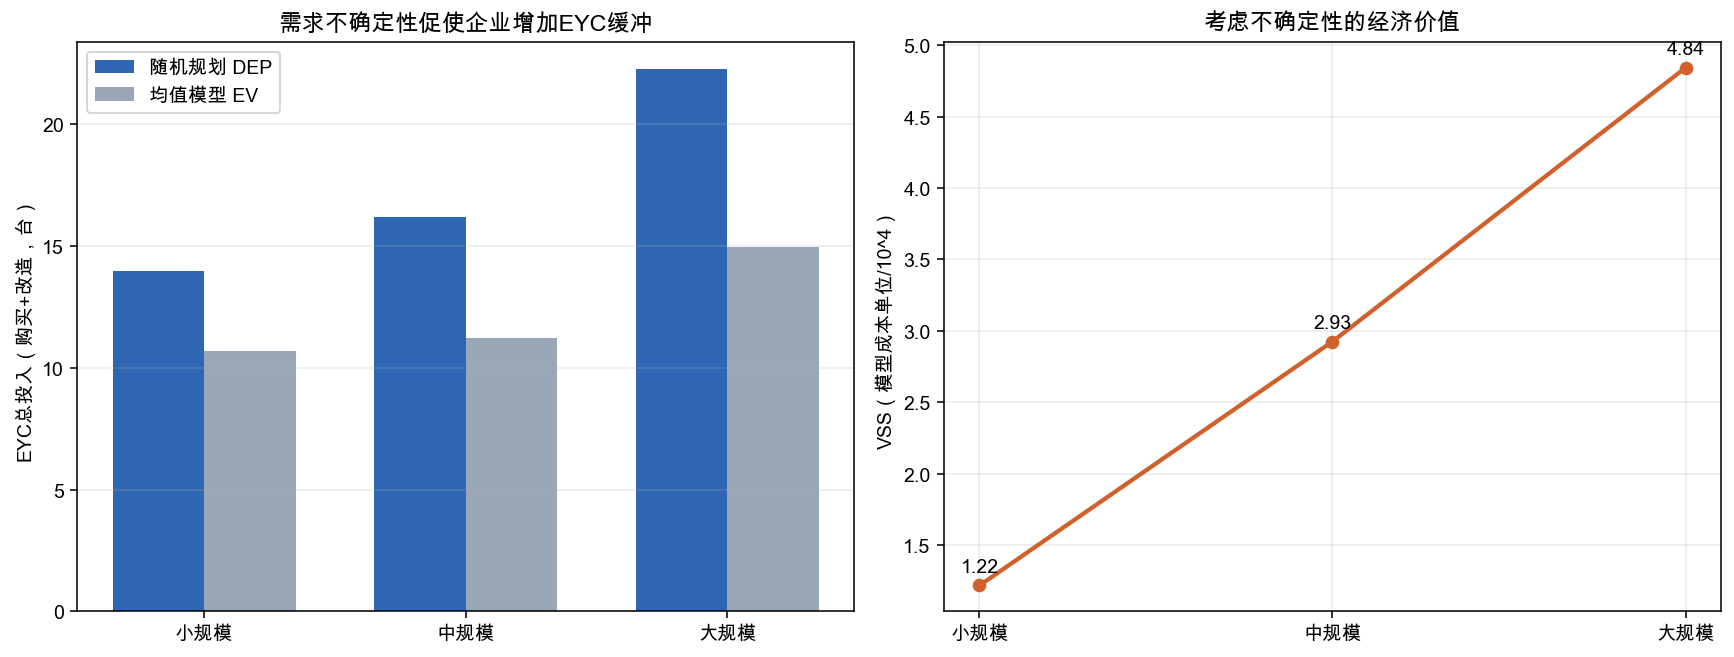
\includegraphics[width=0.92\textwidth]{../main/member3_uncertainty_impact.png}
\caption{随机规划与均值模型的 EYC 投入及 VSS 对比}
\label{fig:member3-uncertainty}
\end{figure}

VSS 均为正，说明随机规划解在真实随机环境下优于均值模型解。其管理含义是：平均需求模型会低估高峰需求的尾部风险，从而低估 EYC 缓冲投入；而随机规划通过同时考虑多个需求场景，将部分运营风险前移到第一阶段投资中处理。

进一步观察不同规模下的结果，可以发现 EYC 增量随问题规模扩大而上升。这一现象并非简单的设备数量扩张，而是由两阶段随机规划的一阶段承诺属性决定的。EYC 购买、DYC 改造和电网铺设都必须在需求实现之前完成，一旦需求高峰出现，企业无法立即通过临时采购或临时改造补足电动化能力。因此，在随机规划中，高需求场景虽然只占样本场景的一部分，但会通过期望运营成本和碳排放成本影响一阶段投资决策。相比之下，EV 模型只看平均需求路径，会把需求峰值平滑掉，从而得到更低的 EYC 配置。

从运营角度看，更多 EYC 预留带来两类收益。第一，EYC 单位运营成本低于 DYC，在需求高峰时可以减少高成本柴油设备的作业比例；第二，EYC 单位碳排放低于 DYC，有助于控制年度排放和超额排放成本。因此，随机规划选择“多配置一部分 EYC”并不是保守冗余，而是用确定性的前期投入换取随机场景下更稳定的运营成本和排放表现。

\subsection{补贴比例 $k$ 的灵敏度分析}

表\ref{tab:member3-subsidy} 给出了中规模算例下部分补贴率的结果。随着 $k$ 提高，企业承担的投资成本下降，因此目标函数值单调下降；但在当前参数下，$k=0$ 到 $k=0.9$ 的最优 EYC 投入和期望总排放几乎不变，直到 $k=1.0$ 时 EYC 投入才从 16.19 台上升至 17.20 台。

\begin{table}[htbp]
\centering
\caption{补贴比例 $k$ 的灵敏度分析（中规模，CV=0.15）}
\label{tab:member3-subsidy}
\begin{tabular}{rrrrrr}
\toprule
$k$ & 目标函数值 & 期望总排放 & 政府补贴支出 & 改造区域数 & EYC投入 \\
\midrule
0.0 & 1855333.86 & 1081.98 & 0.00 & 3.0 & 16.19 \\
0.2 & 1855133.07 & 1081.98 & 200.79 & 3.0 & 16.19 \\
0.5 & 1854831.90 & 1081.98 & 501.96 & 3.0 & 16.19 \\
0.8 & 1854530.72 & 1081.98 & 803.14 & 3.0 & 16.19 \\
1.0 & 1854329.93 & 1081.98 & 1111.92 & 3.0 & 17.20 \\
\bottomrule
\end{tabular}
\end{table}

\begin{figure}[htbp]
\centering
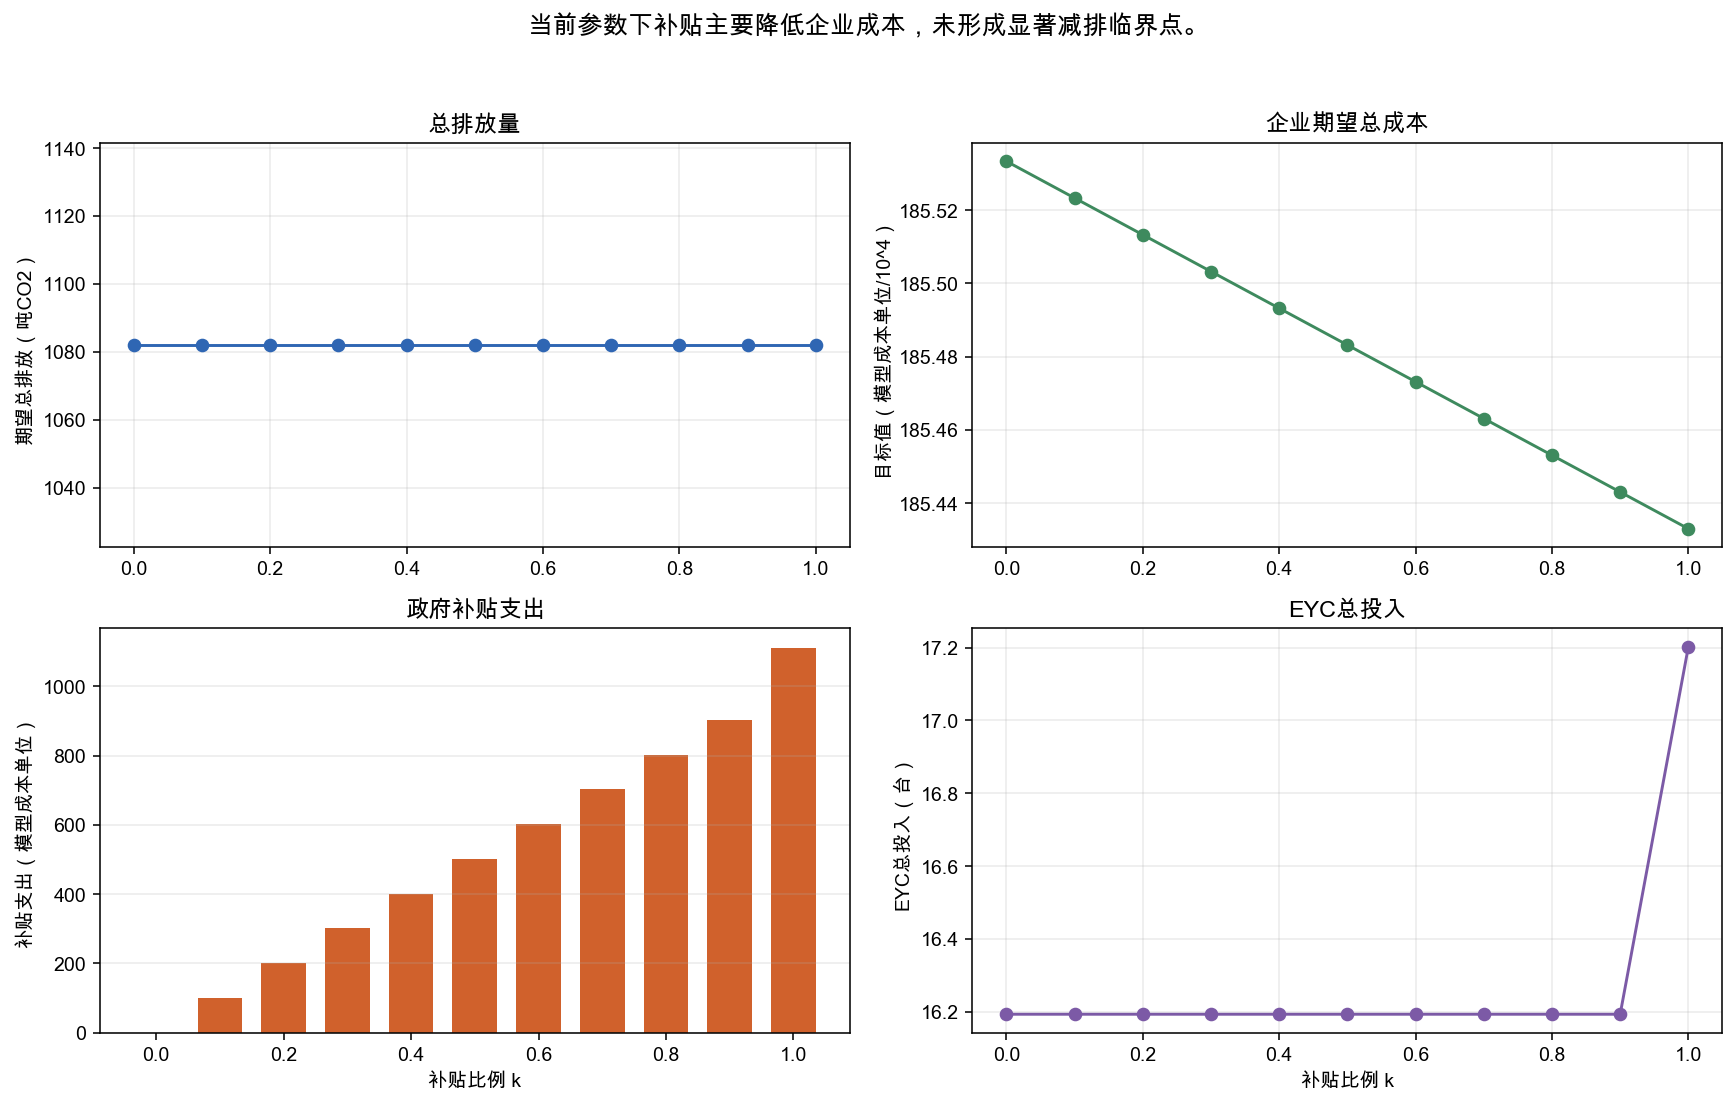
\includegraphics[width=0.92\textwidth]{../main/member3_subsidy_sensitivity.png}
\caption{补贴比例对企业成本、排放、补贴支出与 EYC 投入的影响}
\label{fig:member3-subsidy}
\end{figure}

按照“总排放相对 $k=0$ 下降至少 0.5\%”的标准，本实验未观察到显著减排临界点。电网改造区域数在所有补贴水平下均保持为 3 个，说明基准参数下各区域电网改造已具备经济合理性，补贴并未进一步改变“是否改造区域”的边界。其原因是当前基准参数下，EYC 投资已经主要由运营成本节省和碳成本约束共同驱动；单独提高固定投资补贴更多表现为企业成本向政府预算的转移，而不是立即改变运营排放结构。

这一结果说明，补贴政策的作用存在阶段性差异。当企业原本不愿意改造时，补贴可以通过降低固定投资成本跨过投资门槛；但在本文基准参数下，电网改造和 EYC 配置即使在 $k=0$ 时也已经被模型选择，因此继续提高 $k$ 主要降低企业承担的目标成本。换言之，补贴在这里更像是“成本分担工具”，而不是“边际减排激励工具”。只有当补贴能够改变设备组合、作业分配或改造区域数量时，才会表现为明显的减排临界点。

需要注意的是，$k=1.0$ 时 EYC 投入出现小幅增加，但总排放仍没有明显下降。这是因为新增 EYC 并不必然转化为更多 EYC 作业量：作业分配还受到区域需求、设备产能、电网完成时间、已有 DYC 存量和容量上限约束共同影响。当电动化能力已经能够覆盖主要低成本作业机会时，继续增加 EYC 可能更多表现为备用产能或期末存量增加，而不会立即改变总作业量的排放结构。

因此，若政策制定者的目标是降低企业改造负担，单一投资补贴是有效的；若目标是进一步降低总排放，则仅提高 $k$ 可能不够。更有效的政策组合应同时作用于运营侧，例如提高碳交易价格、加快免费配额递减、设定最低 EYC 作业比例或对实际减排量给予绩效型补贴。

\subsection{不同不确定性水平下的补贴边际效用}

进一步改变需求波动水平后，结果显示 CV 越高，企业为了应对高峰需求配置的 EYC 越多：当 $k=0$ 时，CV=0.05、0.15、0.30 对应的 EYC 投入分别为 12.63、16.19、22.74 台。这说明需求不确定性本身会强化企业的缓冲投资动机。

\begin{table}[htbp]
\centering
\caption{不同需求波动水平下的 EYC 投入与排放响应}
\label{tab:member3-cv}
\begin{tabular}{rrrrr}
\toprule
CV & $k=0$ EYC投入 & $k=1$ EYC投入 & $k=0$ 排放 & $k=1$ 排放 \\
\midrule
0.05 & 12.63 & 30.49 & 1077.77 & 1077.77 \\
0.15 & 16.19 & 17.20 & 1081.98 & 1081.98 \\
0.30 & 22.74 & 35.83 & 1091.99 & 1091.99 \\
\bottomrule
\end{tabular}
\end{table}

\begin{figure}[htbp]
\centering
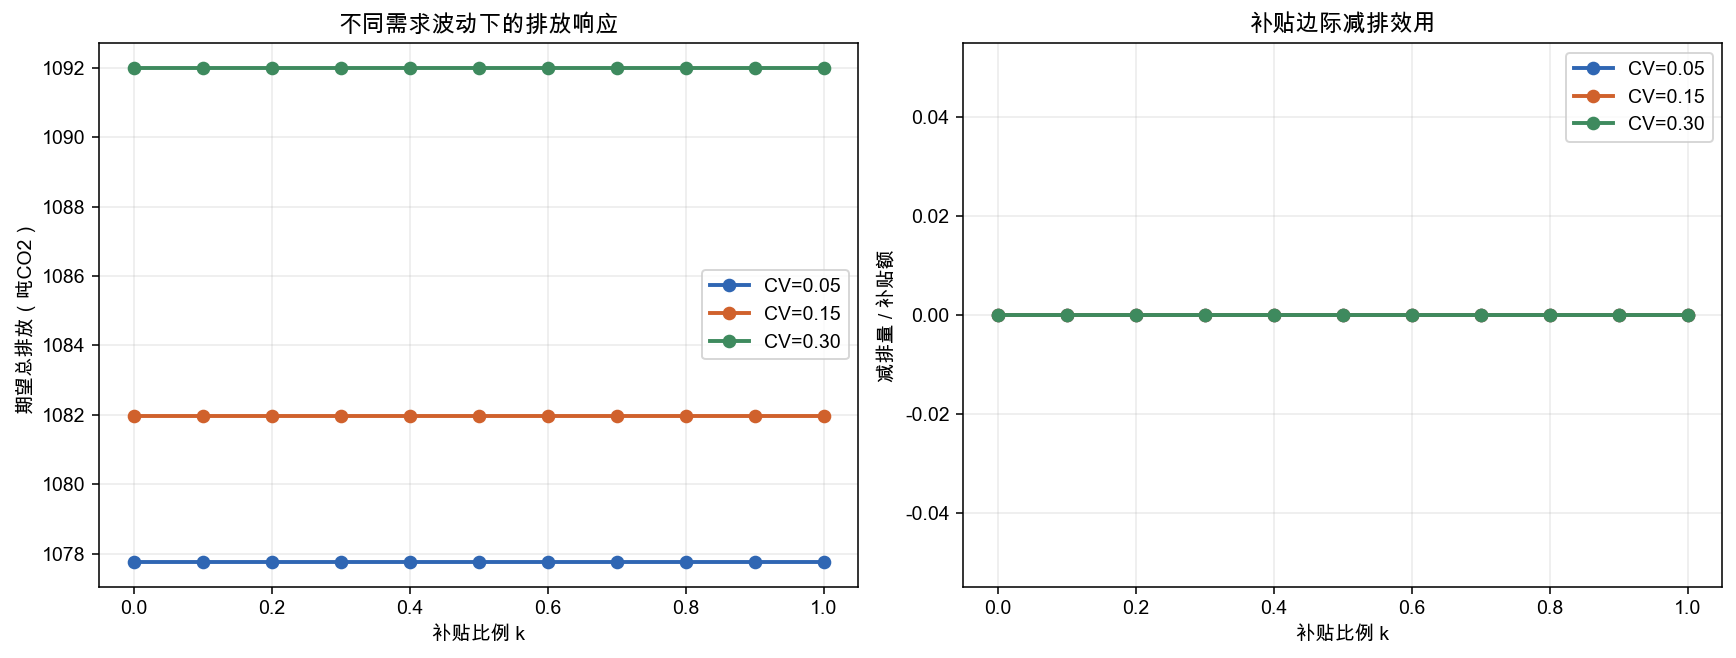
\includegraphics[width=0.92\textwidth]{../main/member3_cv_marginal_effect.png}
\caption{不同 CV 水平下补贴的排放响应与边际减排效用}
\label{fig:member3-cv}
\end{figure}

从政策角度看，单一补贴工具并不一定能在所有参数区间带来额外减排。若政策目标是降低总排放，而不是单纯降低企业改造负担，则补贴应与更高碳交易价格、更严格免费配额递减规则或设备最低电动化比例配合使用。否则，当企业在无补贴条件下已经因为运营经济性而选择电动化时，继续提高补贴的边际减排效用会下降。

CV 扩展实验还揭示了补贴政策与需求不确定性的关系。低波动情形下，企业面对的需求路径较稳定，一阶段投资可以较好地贴合平均需求；高波动情形下，需求峰值出现的概率和幅度上升，企业为了避免高峰期产能不足，会提前配置更多 EYC。因此，需求不确定性越强，企业对电动化设备的“保险性需求”越高。

但是，较高 CV 并不自动意味着补贴具有更强减排效果。表\ref{tab:member3-cv} 中，CV 从 0.05 提高到 0.30 时，$k=0$ 下的 EYC 投入明显增加，但 $k=0$ 与 $k=1$ 的排放水平仍基本一致。这说明不确定性首先改变的是投资规模，而不是必然改变实际作业排放。若要使补贴在高不确定性下产生更强减排效果，需要将补贴发放条件与实际运营行为绑定，例如将补贴与 EYC 作业占比、实际减排吨数或高峰期清洁设备使用率挂钩。

\subsection{实验结论与管理启示}

综合上述结果，可以得到以下结论：
\begin{itemize}[itemsep=0.2em,leftmargin=2em]
    \item 需求不确定性会显著提高企业的一阶段 EYC 缓冲投入，随机规划相比均值模型具有稳定的正 VSS。
    \item 补贴率提高能够降低企业承担的总成本，但在当前参数下未形成显著的排放下降临界点。
    \item 需求波动水平越高，企业越倾向于预留 EYC；补贴政策在高不确定性下更容易扩大设备电动化投入，但减排效果仍取决于作业分配和碳价格等运营侧参数。
\end{itemize}

总体而言，本实验支持一个更细分的政策判断：投资补贴适合解决前期改造成本高、企业现金流压力大的问题；碳交易价格和排放配额规则更适合持续影响运营阶段的设备使用结构。对于港口设备电动化改造，较优的政策设计不应只关注“补贴比例多高”，还应关注补贴是否能触发额外改造、是否能引导 EYC 被实际用于高排放替代场景，以及是否与碳市场信号形成一致激励。

\end{document}
